\documentclass{article}\usepackage[]{graphicx}\usepackage[]{color}
% maxwidth is the original width if it is less than linewidth
% otherwise use linewidth (to make sure the graphics do not exceed the margin)
\makeatletter
\def\maxwidth{ %
  \ifdim\Gin@nat@width>\linewidth
    \linewidth
  \else
    \Gin@nat@width
  \fi
}
\makeatother

\definecolor{fgcolor}{rgb}{0.345, 0.345, 0.345}
\newcommand{\hlnum}[1]{\textcolor[rgb]{0.686,0.059,0.569}{#1}}%
\newcommand{\hlstr}[1]{\textcolor[rgb]{0.192,0.494,0.8}{#1}}%
\newcommand{\hlcom}[1]{\textcolor[rgb]{0.678,0.584,0.686}{\textit{#1}}}%
\newcommand{\hlopt}[1]{\textcolor[rgb]{0,0,0}{#1}}%
\newcommand{\hlstd}[1]{\textcolor[rgb]{0.345,0.345,0.345}{#1}}%
\newcommand{\hlkwa}[1]{\textcolor[rgb]{0.161,0.373,0.58}{\textbf{#1}}}%
\newcommand{\hlkwb}[1]{\textcolor[rgb]{0.69,0.353,0.396}{#1}}%
\newcommand{\hlkwc}[1]{\textcolor[rgb]{0.333,0.667,0.333}{#1}}%
\newcommand{\hlkwd}[1]{\textcolor[rgb]{0.737,0.353,0.396}{\textbf{#1}}}%
\let\hlipl\hlkwb

\usepackage{framed}
\makeatletter
\newenvironment{kframe}{%
 \def\at@end@of@kframe{}%
 \ifinner\ifhmode%
  \def\at@end@of@kframe{\end{minipage}}%
  \begin{minipage}{\columnwidth}%
 \fi\fi%
 \def\FrameCommand##1{\hskip\@totalleftmargin \hskip-\fboxsep
 \colorbox{shadecolor}{##1}\hskip-\fboxsep
     % There is no \\@totalrightmargin, so:
     \hskip-\linewidth \hskip-\@totalleftmargin \hskip\columnwidth}%
 \MakeFramed {\advance\hsize-\width
   \@totalleftmargin\z@ \linewidth\hsize
   \@setminipage}}%
 {\par\unskip\endMakeFramed%
 \at@end@of@kframe}
\makeatother

\definecolor{shadecolor}{rgb}{.97, .97, .97}
\definecolor{messagecolor}{rgb}{0, 0, 0}
\definecolor{warningcolor}{rgb}{1, 0, 1}
\definecolor{errorcolor}{rgb}{1, 0, 0}
\newenvironment{knitrout}{}{} % an empty environment to be redefined in TeX

\usepackage{alltt}

\usepackage{float}
\usepackage{hyperref}

% Set the margins on the page to not be so large
\addtolength{\oddsidemargin}{-.875in}
\addtolength{\evensidemargin}{-.875in}
\addtolength{\textwidth}{1.75in}
\addtolength{\topmargin}{-.875in}
\addtolength{\textheight}{1.75in}

% Take off page numbering
\pagenumbering{gobble}
\IfFileExists{upquote.sty}{\usepackage{upquote}}{}
\begin{document}

\title{%
  5.3 - R: Logistic Regression Case Study \\
  \smallskip
  \large Stat 5100: Dr. Bean
}
\date{}

\maketitle

See 1:15-2:10 of \href{www.youtube.com/watch?v=j4JOjcDFtBE}{www.youtube.com/watch?v=j4JOjcDFtBE}

and 3:31-4:22 of \href{www.youtube.com/watch?v=gEjXjfxoNXM}{www.youtube.com/watch?v=gEjXjfxoNXM}

(full text here:
\href{http://millercenter.org/scripps/archive/speeches/detail/3413}{http://millercenter.org/scripps/archive/speeches/detail/3413})

The January 18, 1986 explosion of the space shuttle Challenger was investigated by the
Presidential Commission on the Space Shuttle Challenger Accident. The Commission's
1986 report attributed the explosion to a burn through of an O-ring seal at a field joint in
one of the solid-fuel rocket boosters. This 1986 launch was the 25th space shuttle launch.
After each of the previous 24 launches, the solid rocket boosters were inspected.
The following data are from the Commission's 1986 report, with the following variables:

\begin{center}
\begin{tabular}{|c|p{8cm}|}
\hline
Flight & an identifier code for the launch \\
\hline
Temp & temperature (degrees F) at launch \\
\hline
Damage & indicator of damage to the field joint (a missing value is recorded for one launch where the solid rocket boosters were not recovered) \\
\hline
\end{tabular}
\end{center}

Note that seven of the 24 launches experienced field joint damage but did not explode
like the Challenger. The Challenger launch was Flight STS51L (not in these data)
and the temperature was 31.

\begin{knitrout}
\definecolor{shadecolor}{rgb}{0.969, 0.969, 0.969}\color{fgcolor}\begin{kframe}
\begin{alltt}
\hlkwd{library}\hlstd{(stat5100)}
\hlkwd{data}\hlstd{(shuttle)}

\hlstd{shuttle}
\end{alltt}
\begin{verbatim}
##    Flight Temp Damage
## 1    STS1   66     NO
## 2    STS9   70     NO
## 3  STS51B   75     NO
## 4    STS2   70    YES
## 5  STS41B   57    YES
## 6  STS51G   70     NO
## 7    STS3   69     NO
## 8  STS41C   63    YES
## 9  STS51F   81     NO
## 10   STS4   80   <NA>
## 11 STS41D   70    YES
## 12 STS51I   76     NO
## 13   STS5   68     NO
## 14 STS41G   78     NO
## 15 STS51J   79     NO
## 16   STS6   67     NO
## 17 STS51A   67     NO
## 18 STS61A   75    YES
## 19   STS7   72     NO
## 20 STS51C   53    YES
## 21 STS61B   76     NO
## 22   STS8   73     NO
## 23 STS51D   67     NO
## 24 STS61C   58    YES
\end{verbatim}
\end{kframe}
\end{knitrout}

We will follow the following steps in this case study:

\begin{enumerate}
  \item Visualize the data
  \item Evaluate the probability of damage based on temperature
  \item Check for influential observations and outliers
  \item Calculate the probability of damage at temperature 31 (temperature at Challenger launch)
  \item How is logistic regression different from ANOVA?
\end{enumerate}

\subsection*{1. Visualize the data}

\begin{knitrout}
\definecolor{shadecolor}{rgb}{0.969, 0.969, 0.969}\color{fgcolor}\begin{kframe}
\begin{alltt}
\hlcom{# We will look at the distribution of temperature by damage}
\hlkwd{boxplot}\hlstd{(shuttle}\hlopt{$}\hlstd{Temp} \hlopt{~} \hlstd{shuttle}\hlopt{$}\hlstd{Damage,} \hlkwc{main} \hlstd{=} \hlstr{"Distribution of Temp by Damage"}\hlstd{,}
        \hlkwc{xlab} \hlstd{=} \hlstr{"Damage"}\hlstd{,} \hlkwc{ylab} \hlstd{=} \hlstr{"Temperature"}\hlstd{)}

\hlcom{# Full data, still separated by temperature}
\hlstd{damage_numeric} \hlkwb{<-} \hlkwd{as.numeric}\hlstd{(shuttle}\hlopt{$}\hlstd{Damage} \hlopt{==} \hlstr{"YES"}\hlstd{)}
\hlkwd{plot}\hlstd{(shuttle}\hlopt{$}\hlstd{Temp, damage_numeric,} \hlkwc{main} \hlstd{=} \hlstr{"Full Data"}\hlstd{,} \hlkwc{xlab} \hlstd{=} \hlstr{"Temperature at launch"}\hlstd{,}
     \hlkwc{ylab} \hlstd{=} \hlstr{"Damage of field joint (1.0 = YES, 0.0 = NO)"}\hlstd{,} \hlkwc{pch} \hlstd{=} \hlnum{16}\hlstd{)}
\end{alltt}
\end{kframe}

{\centering 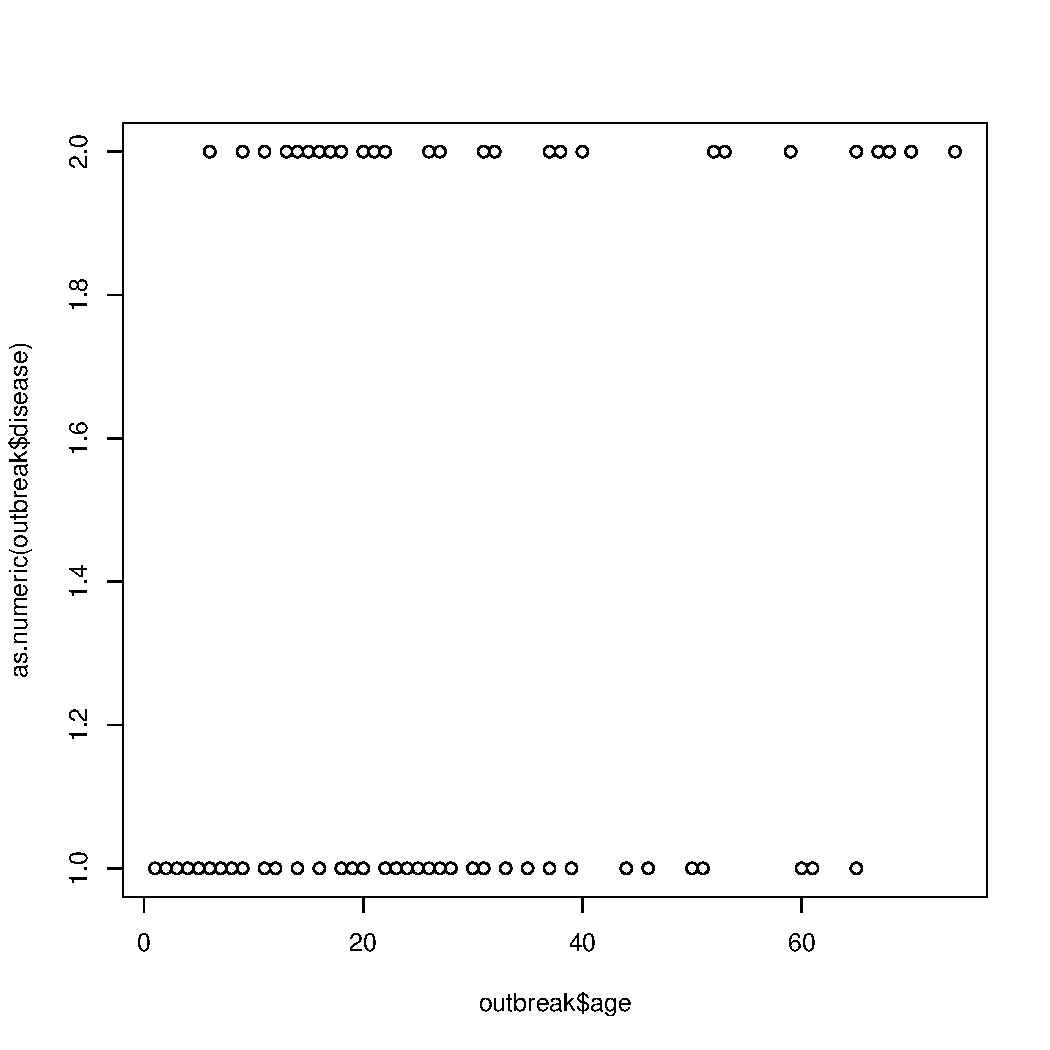
\includegraphics[width=0.45\textwidth]{figure/unnamed-chunk-2-1} 
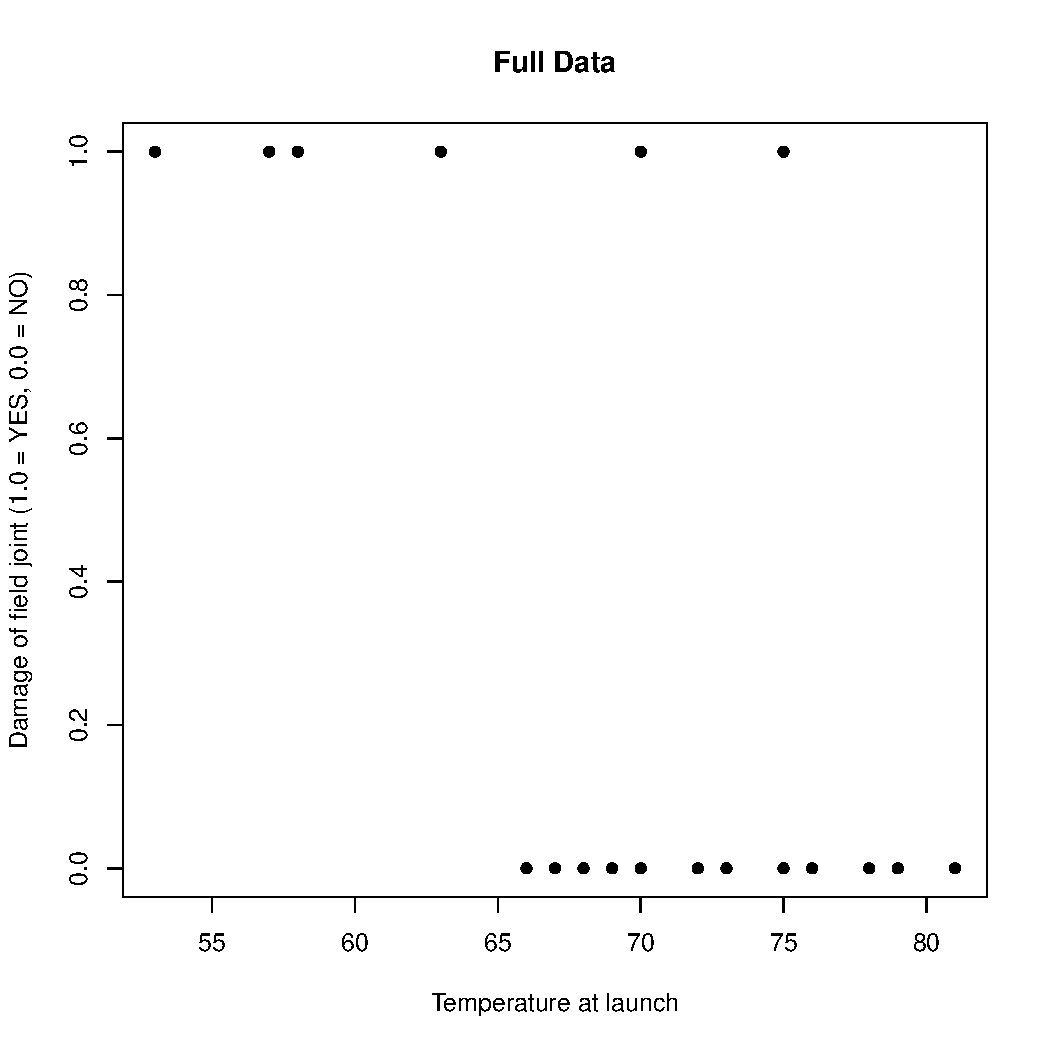
\includegraphics[width=0.45\textwidth]{figure/unnamed-chunk-2-2} 

}



\end{knitrout}

Based upon the above visualizations, we would conclude that damage mostly occurred to the field joint at lower temperatures.

\subsection*{2. Evaluate the probability of damage based on temperature}

\begin{knitrout}
\definecolor{shadecolor}{rgb}{0.969, 0.969, 0.969}\color{fgcolor}\begin{kframe}
\begin{alltt}
\hlcom{# Convert damage to factor type first}
\hlstd{shuttle}\hlopt{$}\hlstd{Damage} \hlkwb{<-} \hlkwd{as.factor}\hlstd{(shuttle}\hlopt{$}\hlstd{Damage)}

\hlstd{shuttle_logreg} \hlkwb{<-} \hlkwd{glm}\hlstd{(Damage} \hlopt{~} \hlstd{Temp,} \hlkwc{data} \hlstd{= shuttle,}
                      \hlkwc{family} \hlstd{=} \hlstr{"binomial"}\hlstd{)}
\hlkwd{summary}\hlstd{(shuttle_logreg)}
\end{alltt}
\begin{verbatim}
## 
## Call:
## glm(formula = Damage ~ Temp, family = "binomial", data = shuttle)
## 
## Deviance Residuals: 
##     Min       1Q   Median       3Q      Max  
## -1.0611  -0.7613  -0.3783   0.4524   2.2175  
## 
## Coefficients:
##             Estimate Std. Error z value Pr(>|z|)  
## (Intercept)  15.0429     7.3786   2.039   0.0415 *
## Temp         -0.2322     0.1082  -2.145   0.0320 *
## ---
## Signif. codes:  0 '***' 0.001 '**' 0.01 '*' 0.05 '.' 0.1 ' ' 1
## 
## (Dispersion parameter for binomial family taken to be 1)
## 
##     Null deviance: 28.267  on 22  degrees of freedom
## Residual deviance: 20.315  on 21  degrees of freedom
##   (1 observation deleted due to missingness)
## AIC: 24.315
## 
## Number of Fisher Scoring iterations: 5
\end{verbatim}
\end{kframe}
\end{knitrout}

Now, let's create a fit plot showing the probability of damage for various levels of temperature.

\begin{knitrout}
\definecolor{shadecolor}{rgb}{0.969, 0.969, 0.969}\color{fgcolor}\begin{kframe}
\begin{alltt}
\hlstd{temp_range} \hlkwb{<-} \hlkwd{seq}\hlstd{(}\hlnum{50}\hlstd{,} \hlnum{85}\hlstd{,} \hlkwc{length.out} \hlstd{=} \hlnum{100}\hlstd{)}
\hlstd{pred_prob_damage} \hlkwb{<-} \hlkwd{predict}\hlstd{(shuttle_logreg,} \hlkwc{newdata} \hlstd{=} \hlkwd{data.frame}\hlstd{(}\hlkwc{Temp} \hlstd{= temp_range),}
                            \hlkwc{type} \hlstd{=} \hlstr{"response"}\hlstd{)}

\hlkwd{plot}\hlstd{(shuttle}\hlopt{$}\hlstd{Temp, damage_numeric,} \hlkwc{main} \hlstd{=} \hlstr{"Predicted probabilities for Damage=YES"}\hlstd{,}
     \hlkwc{xlab} \hlstd{=} \hlstr{"Temperature"}\hlstd{,} \hlkwc{ylab} \hlstd{=} \hlstr{"Probability"}\hlstd{)}
\hlkwd{lines}\hlstd{(temp_range, pred_prob_damage)}
\end{alltt}
\end{kframe}

{\centering 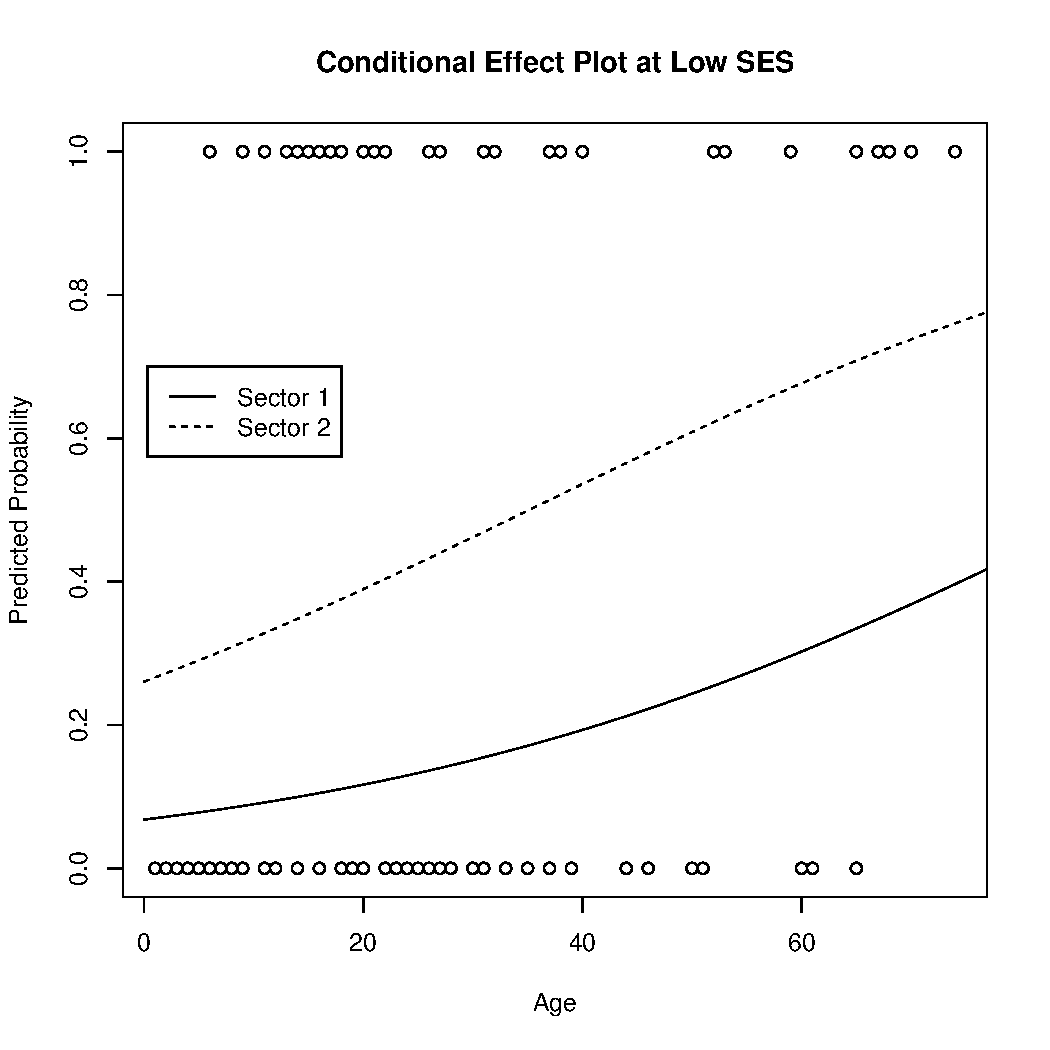
\includegraphics[width=0.6\textwidth]{figure/unnamed-chunk-4-1} 

}



\end{knitrout}

\subsection*{3. Check for influential observations and outliers}

\begin{knitrout}
\definecolor{shadecolor}{rgb}{0.969, 0.969, 0.969}\color{fgcolor}\begin{kframe}
\begin{alltt}
\hlstd{stat5100}\hlopt{::}\hlkwd{logistic_influence_diagnostics}\hlstd{(shuttle_logreg)}
\end{alltt}
\end{kframe}

{\centering 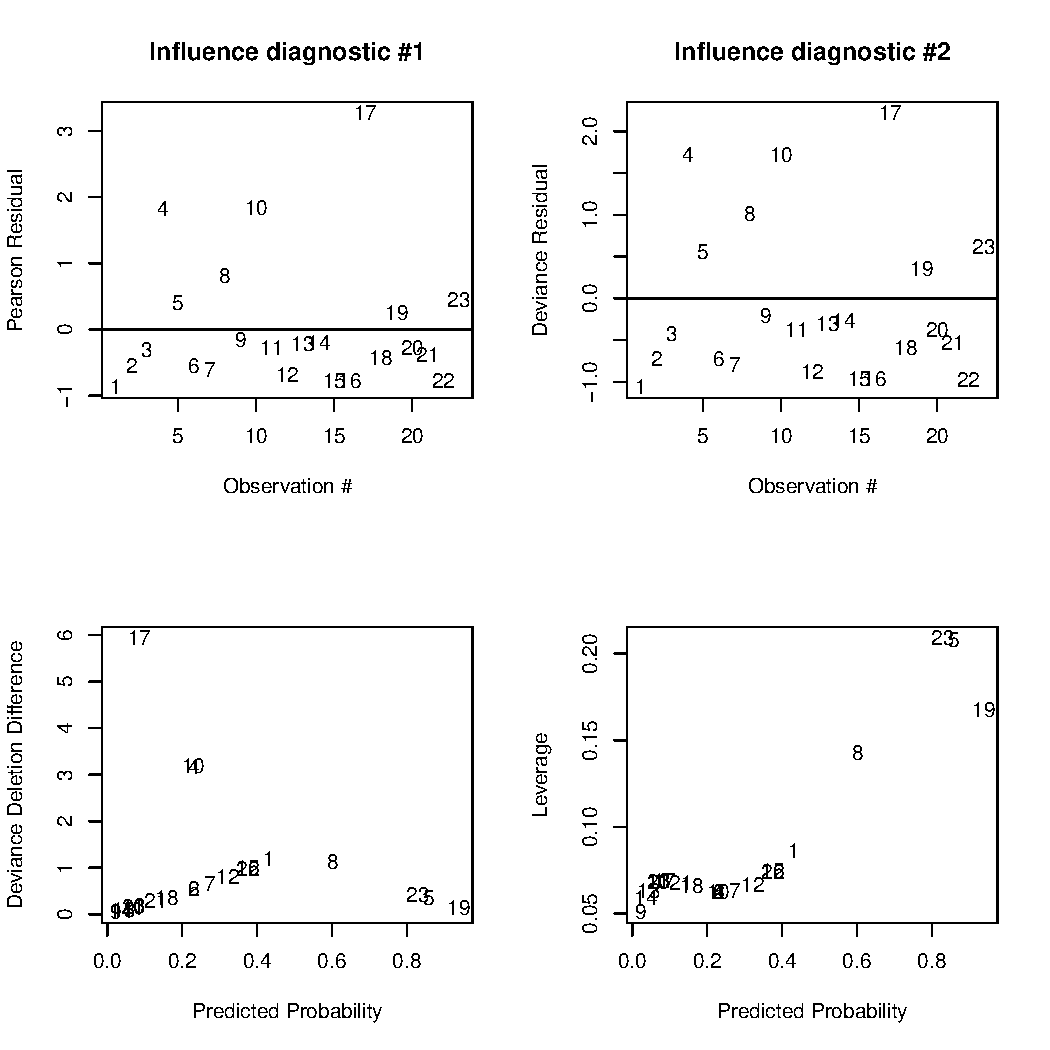
\includegraphics[width=0.6\textwidth]{figure/unnamed-chunk-5-1} 

}



\end{knitrout}

Now let's do an outlier check using the simulated envelope function:

\begin{knitrout}
\definecolor{shadecolor}{rgb}{0.969, 0.969, 0.969}\color{fgcolor}\begin{kframe}
\begin{alltt}
\hlstd{stat5100}\hlopt{::}\hlkwd{simulated_envelope_logreg}\hlstd{(shuttle_logreg)}
\end{alltt}


{\ttfamily\noindent\color{warningcolor}{\#\# Warning: glm.fit: fitted probabilities numerically 0 or 1 occurred}}\end{kframe}

{\centering 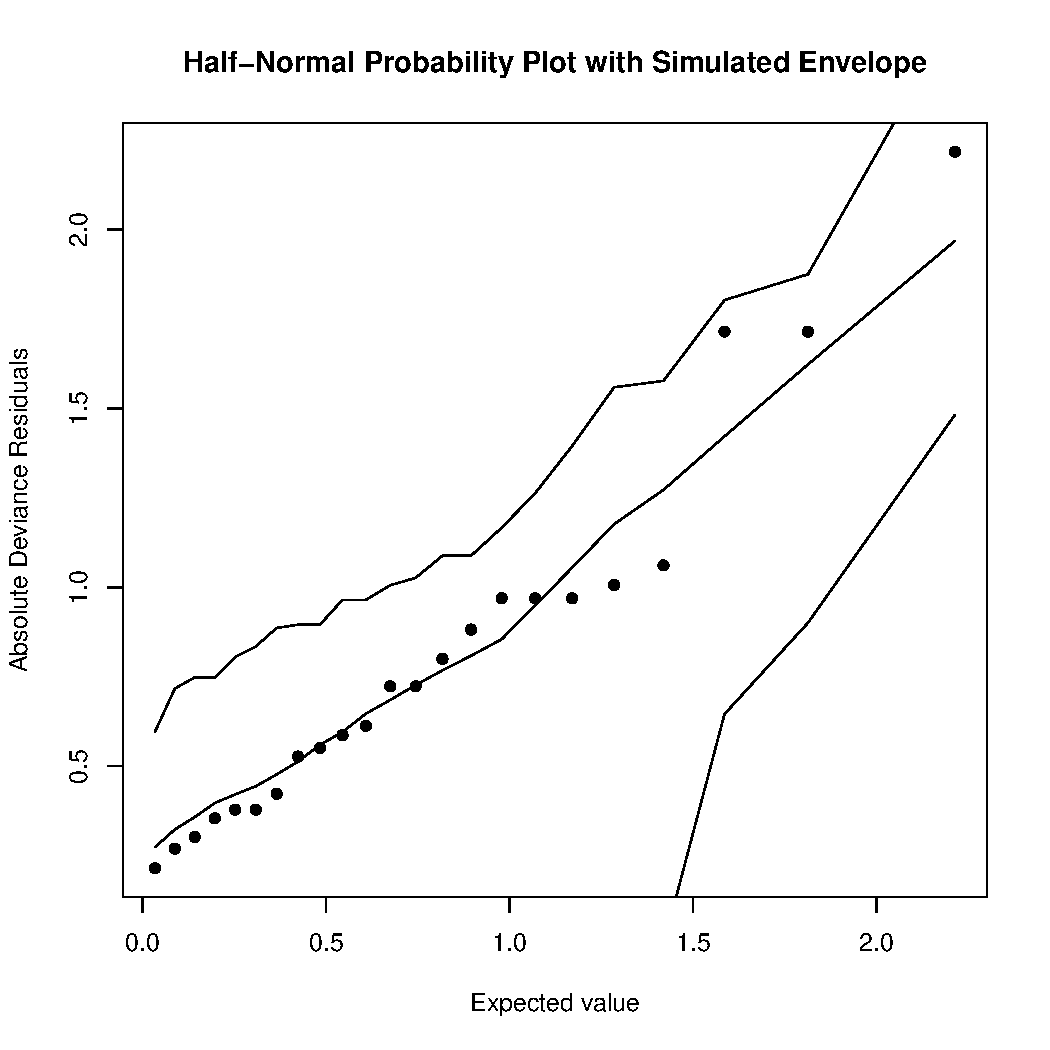
\includegraphics[width=0.6\textwidth]{figure/unnamed-chunk-6-1} 

}



\end{knitrout}

Let's print some suspect observations from the influential diagnostics to get a sense for what types of observations they were:

\begin{knitrout}
\definecolor{shadecolor}{rgb}{0.969, 0.969, 0.969}\color{fgcolor}\begin{kframe}
\begin{alltt}
\hlstd{shuttle[}\hlnum{17}\hlstd{, ]}
\end{alltt}
\begin{verbatim}
##    Flight Temp Damage
## 17 STS51A   67     NO
\end{verbatim}
\begin{alltt}
\hlstd{shuttle[}\hlnum{4}\hlstd{, ]}
\end{alltt}
\begin{verbatim}
##   Flight Temp Damage
## 4   STS2   70    YES
\end{verbatim}
\begin{alltt}
\hlstd{shuttle[}\hlnum{10}\hlstd{, ]}
\end{alltt}
\begin{verbatim}
##    Flight Temp Damage
## 10   STS4   80   <NA>
\end{verbatim}
\end{kframe}
\end{knitrout}

Let's try refitting a model but excluding those observations.

\begin{knitrout}
\definecolor{shadecolor}{rgb}{0.969, 0.969, 0.969}\color{fgcolor}\begin{kframe}
\begin{alltt}
\hlstd{new_shuttle} \hlkwb{<-} \hlstd{shuttle[}\hlopt{-}\hlkwd{c}\hlstd{(}\hlnum{4}\hlstd{,} \hlnum{10}\hlstd{,} \hlnum{17}\hlstd{), ]}
\hlstd{new_shuttle_logreg} \hlkwb{<-} \hlkwd{glm}\hlstd{(Damage} \hlopt{~} \hlstd{Temp,} \hlkwc{data} \hlstd{= new_shuttle,} \hlkwc{family} \hlstd{=} \hlstr{"binomial"}\hlstd{)}
\hlkwd{summary}\hlstd{(new_shuttle_logreg)}
\end{alltt}
\begin{verbatim}
## 
## Call:
## glm(formula = Damage ~ Temp, family = "binomial", data = new_shuttle)
## 
## Deviance Residuals: 
##     Min       1Q   Median       3Q      Max  
## -1.0209  -0.6600  -0.3174   0.3151   2.3535  
## 
## Coefficients:
##             Estimate Std. Error z value Pr(>|z|)  
## (Intercept)  16.6681     8.1242   2.052   0.0402 *
## Temp         -0.2583     0.1198  -2.156   0.0311 *
## ---
## Signif. codes:  0 '***' 0.001 '**' 0.01 '*' 0.05 '.' 0.1 ' ' 1
## 
## (Dispersion parameter for binomial family taken to be 1)
## 
##     Null deviance: 25.127  on 20  degrees of freedom
## Residual deviance: 16.330  on 19  degrees of freedom
## AIC: 20.33
## 
## Number of Fisher Scoring iterations: 5
\end{verbatim}
\end{kframe}
\end{knitrout}

\subsection*{4. Calculate the probability of damage at temperature 31}

\begin{knitrout}
\definecolor{shadecolor}{rgb}{0.969, 0.969, 0.969}\color{fgcolor}\begin{kframe}
\begin{alltt}
\hlkwd{predict}\hlstd{(new_shuttle_logreg,} \hlkwc{newdata} \hlstd{=} \hlkwd{data.frame}\hlstd{(}\hlkwc{Temp} \hlstd{=} \hlkwd{c}\hlstd{(}\hlnum{31}\hlstd{)),} \hlkwc{type} \hlstd{=} \hlstr{"response"}\hlstd{)}
\end{alltt}
\begin{verbatim}
##         1 
## 0.9998268
\end{verbatim}
\end{kframe}
\end{knitrout}

\subsection*{5. How is logistic regression different from ANOVA?}

\begin{knitrout}
\definecolor{shadecolor}{rgb}{0.969, 0.969, 0.969}\color{fgcolor}\begin{kframe}
\begin{alltt}
\hlkwd{anova}\hlstd{(}\hlkwd{lm}\hlstd{(Temp} \hlopt{~} \hlstd{Damage,} \hlkwc{data} \hlstd{= shuttle))}
\end{alltt}
\begin{verbatim}
## Analysis of Variance Table
## 
## Response: Temp
##           Df Sum Sq Mean Sq F value   Pr(>F)   
## Damage     1 344.47  344.47  9.6301 0.005383 **
## Residuals 21 751.18   35.77                    
## ---
## Signif. codes:  0 '***' 0.001 '**' 0.01 '*' 0.05 '.' 0.1 ' ' 1
\end{verbatim}
\begin{alltt}
\hlkwd{summary}\hlstd{(}\hlkwd{lm}\hlstd{(Temp} \hlopt{~} \hlstd{Damage,} \hlkwc{data} \hlstd{= shuttle))}
\end{alltt}
\begin{verbatim}
## 
## Call:
## lm(formula = Temp ~ Damage, data = shuttle)
## 
## Residuals:
##      Min       1Q   Median       3Q      Max 
## -10.7143  -5.1250  -0.7143   4.8750  11.2857 
## 
## Coefficients:
##             Estimate Std. Error t value Pr(>|t|)    
## (Intercept)   72.125      1.495  48.237  < 2e-16 ***
## DamageYES     -8.411      2.710  -3.103  0.00538 ** 
## ---
## Signif. codes:  0 '***' 0.001 '**' 0.01 '*' 0.05 '.' 0.1 ' ' 1
## 
## Residual standard error: 5.981 on 21 degrees of freedom
##   (1 observation deleted due to missingness)
## Multiple R-squared:  0.3144,	Adjusted R-squared:  0.2818 
## F-statistic:  9.63 on 1 and 21 DF,  p-value: 0.005383
\end{verbatim}
\begin{alltt}
\hlcom{# Plot the linear model:}
\hlkwd{plot}\hlstd{(damage_numeric, shuttle}\hlopt{$}\hlstd{Temp,} \hlkwc{xlab} \hlstd{=} \hlstr{"Damage (1=YES, 0=NO)"}\hlstd{,}
     \hlkwc{ylab} \hlstd{=} \hlstr{"Temperature"}\hlstd{,} \hlkwc{main} \hlstd{=} \hlstr{"Fit plot for Temp"}\hlstd{)}
\hlkwd{abline}\hlstd{(}\hlkwc{a} \hlstd{=} \hlnum{72.125}\hlstd{,} \hlkwc{b} \hlstd{=} \hlopt{-}\hlnum{8.411}\hlstd{)}
\end{alltt}
\end{kframe}
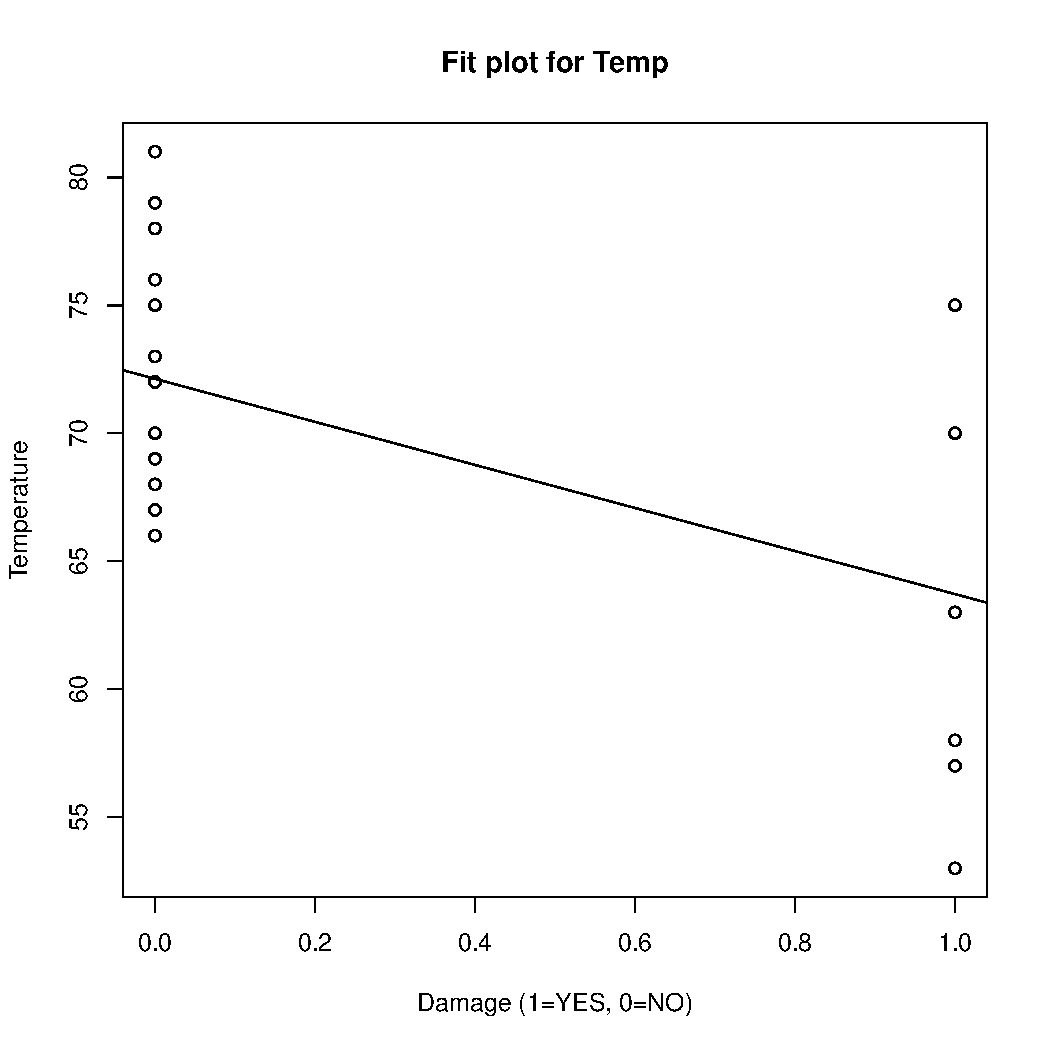
\includegraphics[width=\maxwidth]{figure/unnamed-chunk-10-1} 

\end{knitrout}


\end{document}
